\documentclass[10pt]{article}
\usepackage[spanish]{babel}
\usepackage[utf8]{inputenc}
\usepackage{graphicx} 
\title{M\'etodos abiertos, M\'etodo de la secante}
\author{R\'omulo Walter Condori Bustincio}
\date{}
\begin{document}
\maketitle
\begin{enumerate}
\item para el an\'alisis con el m\'etodo del punto fijo, se considera la siguiente funci\'on $$x^2- 2$$, cuya gr\'afica es la siguiente:
\begin{center}
 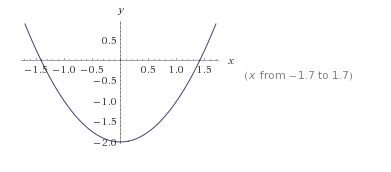
\includegraphics[scale=0.8]{./grafica.jpg}
 % grafica1.jpg: 0x0 pixel, 300dpi, 0.00x0.00 cm, bb=
\end{center}
el algoritmo produce la siguiente salida:\\

Con un total de 36 de 200 iteraciones permitidas, se obtuvo la siguiente tabla:
\begin{center}
\begin{tabular}{|c|c|c|}
\hline
Iteraci\'on&$r$&$f(r)$\\
\hline
1&2&0.111111\\
2&1.8&0.0739857\\
3&1.676&0.0507162\\
4&1.5951&0.0353322\\
5&1.54067&0.0248557\\
6&1.5033&0.0175939\\
7&1.47731&0.0125042\\
8&1.45907&0.00891124\\
9&1.44618&0.00636253\\
10&1.43704&0.00454867\\
11&1.43053&0.00325487\\
12&1.42589&0.00233056\\
13&1.42257&0.0016695\\
14&1.4202&0.00119633\\
15&1.4185&0.000857459\\
16&1.41729&0.000614679\\
17&1.41642&0.000440691\\
18&1.41579&0.000315978\\
19&1.41535&0.000226571\\
20&1.41503&0.00016247\\
21&1.4148&0.000116507\\
22&1.41463&8.35493e-05\\
23&1.41451&5.99156e-05\\
24&1.41443&4.29677e-05\\
25&1.41437&3.08139e-05\\
26&1.41432&2.20981e-05\\
27&1.41429&1.58477e-05\\
28&1.41427&1.13652e-05\\
29&1.41425&8.15057e-06\\
30&1.41424&5.84522e-06\\
31&1.41423&4.19193e-06\\
32&1.41423&3.00627e-06\\
33&1.41422&2.15596e-06\\
34&1.41422&1.54616e-06\\
35&1.41422&1.10884e-06\\
\hline
\end{tabular}
\end{center}
Donde el valor de $r$ aproximado es 1.41422 con un error relativo de: 7.95213e-07

\end{enumerate}
\end{document}


